\renewcommand{\theequation}{\theenumi}
\begin{enumerate}[label=\arabic*.,ref=\thesubsection.\theenumi]
\numberwithin{equation}{enumi}
\item In which of the following situations, does the list of numbers involved make an arithmetic progression, and why?
\begin{enumerate}
\item The taxi fare after each km when the fare is \rupee 15 for the first km and \rupee 8 for each additional km.
\item The amount of air present in a cylinder when a vacuum pump removes 
$\frac{1}{4}$ of the air remaining in the cylinder at a time.
\item  The cost of digging a well after every metre of digging, when it costs \rupee 150 for the first metre and rises by \rupee 50 for each subsequent metre.
\item The amount of money in the account every year, when \rupee 10000 is deposited at compound interest at 8 \% per annum.
\end{enumerate}
\item Write first four terms of the AP, when the first term a and the common difference d are
given as follows:
\begin{enumerate}
\item a = 10, d = 10
\item a = 4, d = –3
\item a = –2, d = 0
\item  a = –1, d =$\frac{1}{2}$
\item a = –1.25, d = –0.25
\end{enumerate}
\item For the following APs, write the first term and the common difference:
\begin{enumerate}
\item 3, 1, –1, –3, . . .
\item –5, –1, 3, 7, . . .
\item $\frac{1}{3}, \frac{5}{3}, \frac{9}{3}, \frac{13}{3},....$
\item 0.6, 1.7, 2.8, 3.9....
\end{enumerate}
\item Which of the following are APs ? If they form an AP, find the common difference d and
write three more terms.
\begin{enumerate}
\item 2, 4, 8, 16, . . .
\item 2,$\frac{5}{2}, 3, \frac{7}{2},...$
\item –1.2, –3.2, –5.2, –7.2, . . .
\item –10, –6, –2, 2, . . .
\item $3,3+\sqrt{2}, 3+2\sqrt{2}, 3+3\sqrt{2},.....$
\item 0.2, 0.22, 0.222, 0.2222, . . .
\item 0, –4, –8, –12, . . .
\item $-\frac{1}{2}, -\frac{1}{2}, -\frac{1}{2}, -\frac{1}{2},....$
\item 1, 3, 9, 27,...
\item a, 2a, 3a, 4a,...
\item $a, a^2, a^3, a^4,...$
\item $\sqrt{2}, \sqrt{8}, \sqrt{18}, \sqrt{32},....$
\item $\sqrt{3}, \sqrt{6}, \sqrt{9}, \sqrt{12},....$
\item $1^2, 3^2, 5^2, 7^2$
\item $1^2, 5^2, 7^2, 73,...$
\end{enumerate}
\item Fill in the blanks in the following table, given that a is the first term, d the common
difference and $a_n$ the $n^{th}$ term of the AP:\\\\
\begin{tabular}{|c|c|r|l|l|}
\hline
&a& d & n & $a_n$\\
\hline
\hline
(i)& 7 &3 &8 &....\\
(ii)& -18 &.... &10  &0\\
(iii)& .... &-3 &18 &-5\\
(iv)& -18.9 &2.5 &.... &3.6\\
(v)& 3.5 &0 &105 &....\\
\hline
\end{tabular}
\item Choose the correct choice in the following and justify :\\
(i) $30^{th}$ term of the AP: 10, 7, 4,..., is
\begin{enumerate}
\item 97
\item 77
\item -77
\item -87
\end{enumerate}
(ii) $11^{th}$ term of the AP: $ -3, -\frac{1}{2}, 2,....,$ is 
\begin{enumerate}
\item 28
\item 22
\item -38
\item $-48\frac{1}{2}$
\end{enumerate}
(iii) In the following APs, find the missing terms in the blanks  :
\begin{enumerate}
\item 2, .... , 26
\item ...., 13. ...., 3
\item 5, ...., ...., 9$\frac{1}{2}$
\item -4, ...., ...., ...., ..., 6
\item ...., 38, ...., ...., ...., -22
\end{enumerate}
\item Which term of the AP : 3, 8, 13, 18, . . . ,is 78?
\item Find the number of terms in each of the following APs:\\
(i) 7, 13, 19, ....,205.\\
(ii) 18, $15\frac{1}{2}, 13,....,-47$
\item Check whether – 150 is a term of the AP : 11, 8, 5, 2 ....
\item Find the 31st term of an AP whose 11th term is 38 and the 16th term is 73.
\item An AP consists of 50 terms of which 3rd term is 12 and the last term is 106. Find the 29th term.
\item If the 3rd and the 9th terms of an AP are 4 and -8 respectively, which term of this AP is zero?
\item The 17th term of an AP exceeds its 10th term by 7. Find the common difference.
\item Which term of the AP : 3, 15, 27, 39,... will be 132 more than its 54th term? 
\item Two APs have the same common difference. The difference between their 100th terms is 100, what is the difference between their 1000th terms?
\item How many three-digit numbers are divisible by 7?
\item How many multiples of 4 lies between 10 and 250?
\item For what value of n, are the $n^{th}$ terms of two APs: 63, 65, 67,.... and 3, 10, 17,... equal?
\item Determine the AP whose third term is 16 and the 7th term exceeds the 5th term by 12.
\item Find the 20th term from the last term of the AP : 3, 8, 13,..., 253.
\item The sum of the 4th and 8th terms of an AP is 24 and the sum of the 6th and 10th terms is 44. Find the first three terms of the AP.
\item Subba Rao started work in 1995 at an annual salary of \rupee 5000 and received an increment of \rupee 200 each year. In which year did his income reach \rupee 7000?
\item Ramkali saved \rupee 5 in the first week of a year and then increased her weekly savings by \rupee 1.75. If in the $n^{th}$ week, her weekly savings become \rupee 20.75, find n.
\item Find the sum of the following APs:\\
(i) 2, 7, 12, . . ., to 10 terms.\\
(ii) -37, -33, -29, . . ., to 12 terms.\\
(iii) 0.6, 1.7, 2.8, . . ., to 100 terms.\\
(iv) $\frac{1}{15}, \frac{1}{12}, \frac{1}{10},.....,$ to 11 terms.
\item Find the sums given below :\\
(i) $7+10\frac{1}{2}+14+...+84$\\
(ii) 34 + 32 + 30 + . . . + 10\\
(iii) -5 + (-8) + (-11) + . . . + (-230)
\item In an A.P:\\
(i) given a = 5, d = 3, $a_n$ = 50, find n and $S_n.$\\
(ii) given a = 7, $a_{13}$ = 35, find d and $S_{13}.$\\
(iii) given $a_{12}$ = 37, d = 3, find a and $S_{12}.$\\
(iv) given $a_3$ = 15, $S_{10}$ = 125, find d and $a_{10}.$\\
(v) given d = 5, $S_9$= 75, find a and $a_9.$\\
(vi) given a = 2, d = 8, $S_n$ = 90, find n and $a_n.$\\
(vii) given a = 8, $a_n$ = 62, $S_n$ = 210, find n and d.\\
(viii) given $a_n$ = 4, d = 2, $S_n$ = –14, find n and a.\\
(ix) given a = 3, n = 8, S = 192, find d.\\
(x) given l = 28, S = 144, and there are total 9 terms. Find a.
\item How many terms of the AP : 9, 17, 25, . . . must be taken to give a sum of 636?
\item The first term of an AP is 5, the last term is 45 and the sum is 400. Find the number of terms and the common difference.
\item The first and the last terms of an AP are 17 and 350 respectively. If the common difference is 9, how many terms are there and what is their sum?
\item Find the sum of first 22 terms of an AP in which d = 7 and 22nd term is 149.
\item Find the sum of first 51 terms of an AP whose second and third terms are 14 and 18 respectively.
\item If the sum of first 7 terms of an AP is 49 and that of 17 terms is 289, find the sum of first n terms. 
\item Show that $a_1 , a_2 , . . ., a_n$ , . . . form an AP where $a_n$ is defined as below :\\
(i) $a_n$ = 3 + 4n\\
(ii) $a_n$ = 9 – 5n\\
Also find the sum of the first 15 terms in each case.
\item If the sum of the first n terms of an AP is 4n - $n^2$ , what is the first term (that is $S_1$ )? What
is the sum of first two terms? What is the second term? Similarly, find the 3rd, the 10th and
the nth terms.
\item Find the sum of the first 40 positive integers divisible by 6.
\item Find the sum of the first 15 multiples of 8.
\item Find the sum of the odd numbers between 0 and 50.
\item A contract on construction job specifies a penalty for delay of completion beyond a
certain date as follows: \rupee 200 for the first day,\rupee 250 for the second day, \rupee 300 for the third
day, etc., the penalty for each succeeding day being \rupee 50 more than for the preceding day. How much money the contractor has to pay as penalty, if he has delayed the work by 30days?
\item A sum of \rupee 700 is to be used to give seven cash prizes to students of a school for their overall academic performance. If each prize is \rupee 20 less than its preceding prize, find the value of each of the prizes.
\item  In a school, students thought of planting trees in and around the school to reduce air pollution. It was decided that the number of trees, that each section of each class will plant, will be the same as the class, in which they are studying, \\
e.g., a section of Class I will plant 1 tree, \\
a section of Class II will plant 2 trees and so on till Class XII.\\ There are three sections of each class. How many trees will be planted by the students?
\item A spiral is made up of successive semicircles, with centres alternately at A and B, starting with centre at A, of radii 0.5 cm, 1.0 cm, 1.5 cm, 2.0 cm,... as shown in Fig. What is the total length of such a spiral made up of thirteen consecutive 22 semicircles? (Take $\pi =\frac{22}{7}$)\\
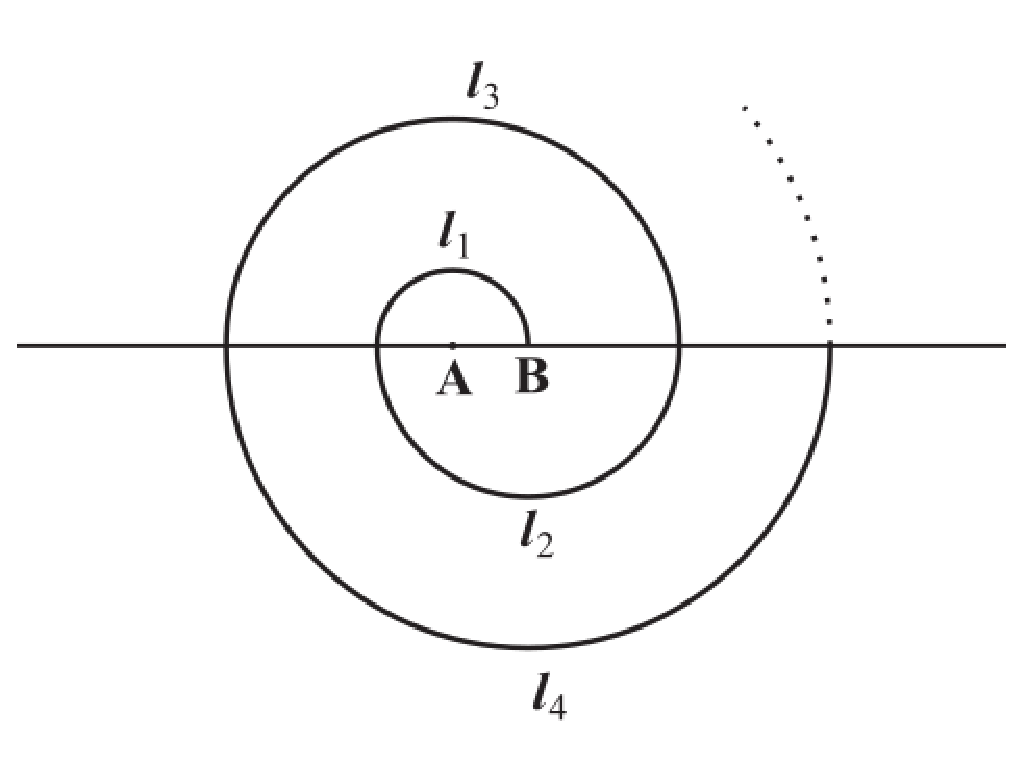
\includegraphics[width=\columnwidth]{./figs/fig.eps} \\
\textbf{Hint :} Length of successive semicircles is $l_1, l_2, l_3, l_4 , . . .$ with centres at A, B, A, B, . . .,respectively.
\item 200 logs are stacked in the following manner: 20 logs in the bottom row, 19 in the next row, 18 in the row next to it and so on (see Fig). In how many rows are the 200 logs placed and how many logs are in the top row?\\
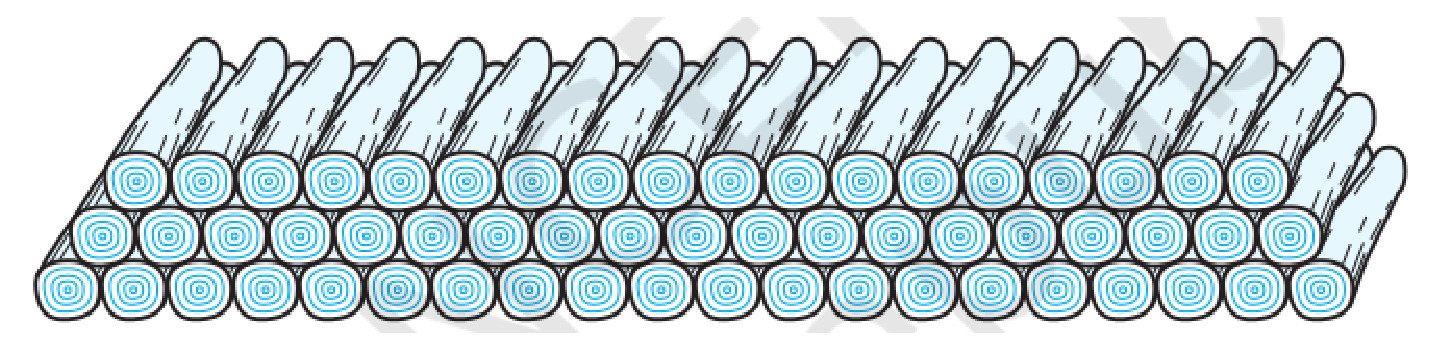
\includegraphics[width=\columnwidth]{./figs/fig1.eps} \\
\item In a potato race, a bucket is placed at the starting point, which is 5m from the first potato, and the other potatoes are placed 3m apart in a straight line. There are ten potatoes in the line.
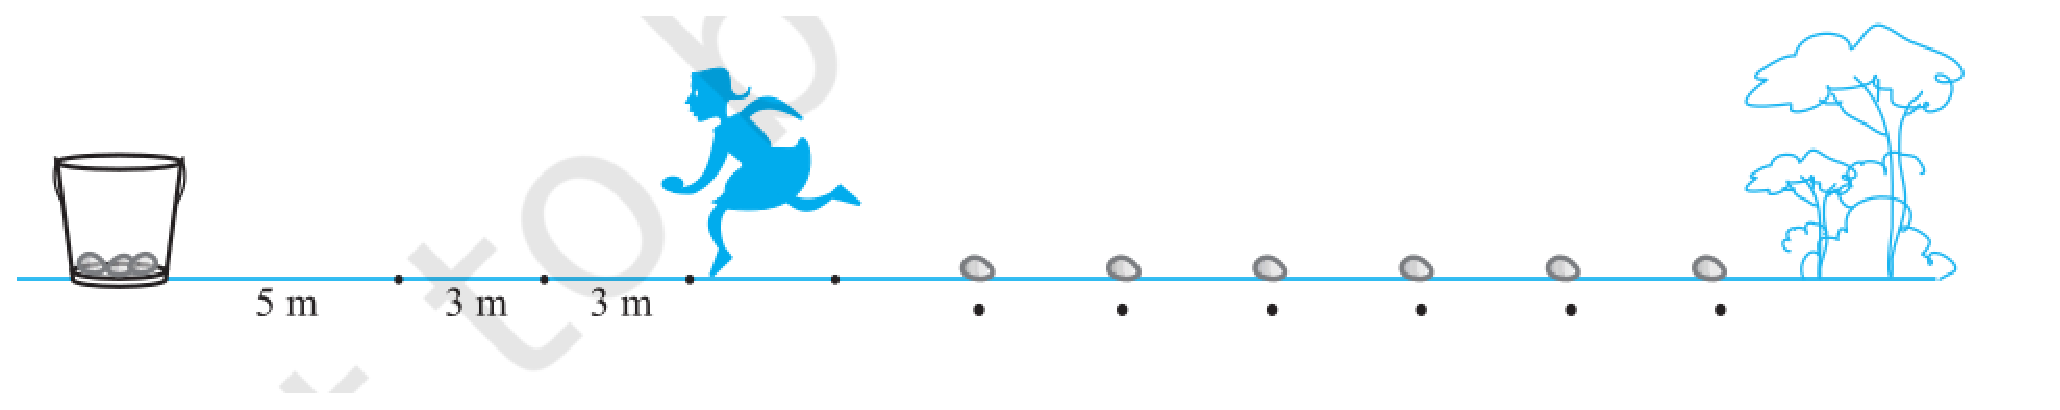
\includegraphics[width=\columnwidth]{./figs/fig3.eps} 
A competitor starts from the bucket, picks up the nearest potato, runs back with it, drops it in the bucket, runs back to pick up the next potato, runs to the bucket to drop it in, and she continues in the same way until all the potatoes are in the bucket. What is the total distance the competitor has to run?\
[\textbf{Hint} : To pick up the first potato and the second potato, the total distance (in metres)
run by a competitor is 2 $\times$ 5 + 2 $\times$ (5 + 3)].
\item Which term of the AP :121, 117, 113,...,is its first negative term?[\textbf{Hint:}Find n for a n $<$ 0]
\item The sum of the third and the seventh terms of an AP is 6 and their product is 8. Find the sum of first sixteen terms of the AP.
\item A ladder has rungs 25 cm apart. The rungs decrease uniformly in length from 45 cm at the bottom to 25 cm at the top. If the top and the bottom rungs are $2\frac{1}{2}$m apart, which is the length of the wood required for the rungs?[\textbf{Hints:} Number of rungs = $\frac{250}{25}+1$]\\
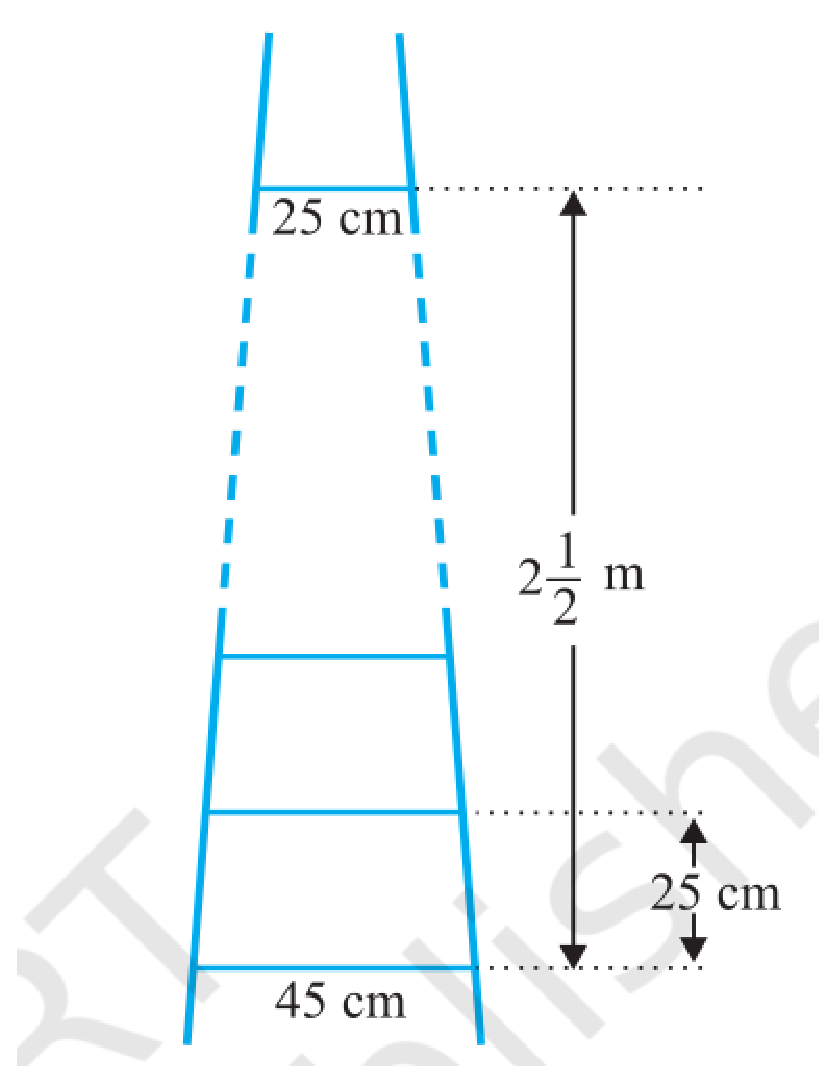
\includegraphics[width=\columnwidth]{./figs/fig4.eps} 
\item The houses of a row are numbered consecutively from 1 to 49. Show that there is a value of x such that the sum of the numbers of the houses preceding the house numbered x is equal to the sum of the numbers of the houses following it. Find this value of x.[\textbf{Hint:} $S_{X-1} = S_49 -S-x$]
\item A small terrace at a football ground comprises of 15 steps each of which is 50 m long and built of solid concrete. Each step has rise of $\frac{1}{4}$m and a tread of $\frac{1}{2}$m .Caluculate the total volume of concrete required to build the terrace.[\textbf{Hint:} Volume of concrete required to build the first step =$\frac{1}{4}X \frac{1}{2}X 50m^3$]\\
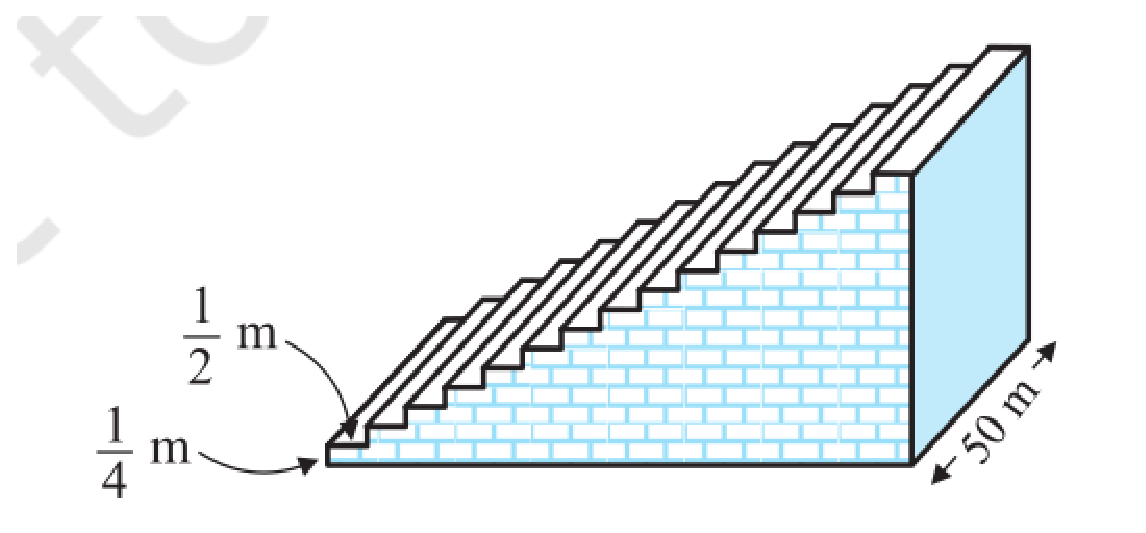
\includegraphics[width=\columnwidth]{./figs/fig5.eps}  
\end{enumerate}
%\end{document}
    
